\section{Experimental Results \& Evaluation}
\label{sec:eval}

This section reports the test results for our agents across Levels~1--7. We compare two learning algorithms, two training modes, and three reward settings, and then look at sample efficiency, failure causes, and how well the saved agents work on new maps.

\subsection{Setup}
\label{subsec:setup}

We run all experiments on Levels~1--7 of \textit{Ho{\'a}'s Midnight Escape}. (The training script ran Levels~1--8 sequentially, and this evaluation focuses on the 7 core levels.) Each level runs for $10{,}000$ episodes, giving $70{,}000$ episodes across Levels~1--7. Every setting is repeated with $8$ independent random seeds ($42$ to $49$), which control both the agent and the environment.

We compare two agents: \textbf{Tabular Q-Learning} (which updates with the max next Q-value) and \textbf{Hybrid Expected SARSA} (which weights the next Q-values by the $\epsilon$-greedy policy). Both agents are tested in two training modes:
\begin{itemize}
    \item \textbf{Curriculum}: One Q-table starts on Level~1 and keeps training from Level~1 through Level~7. When entering a new level, exploration $\epsilon$ re-warms to at least $0.30$ on Levels~2--3 and $0.35$ on Levels~4--7. To reduce forgetting, after Level~1 the trainer also runs background replay episodes on earlier levels in round-robin order (configured with \texttt{replay\_ratio} $= 0.35$, implemented in \texttt{training/trainer.py} as a $\max(0.35, 0.5) = 0.50$ chance per episode of one greedy replay on a prior level, alongside replay of up to 5 stored winning paths).
    \item \textbf{Separate}: A fresh Q-table starts from scratch on each level with $\epsilon = 1.0$, without carry-over or prior-level replay.
\end{itemize}

We also test three reward functions: \textbf{Balanced} (our main shaped reward with forward/backward progress, item bonuses, hazard-timing guidance, and strong death/timeout penalties), \textbf{Dense} (goal-distance progress shaping with weaker penalties and no hazard-timing terms), and \textbf{Sparse} (only terminal goal/death signals and item bonuses).

For Levels~4--7, \texttt{training/trainer.py} uses a reverse-spawn schedule so the agent first practices closer to the goal and then moves back toward the start. In Curriculum mode, spawns step backward through fractions $(0.80, 0.60, 0.40, 0.20)$ of the goal distance before reaching the normal start, advancing when the agent passes a greedy check every 25 episodes or hits $1{,}428$ episodes in a segment (with $\epsilon$ reset to $0.30$ or $0.25$ and decay $0.985$ during reverse segments). In Separate mode, spawns follow fixed blocks of the $10{,}000$ episodes: $0.75$ of goal distance for episodes $1$--$1{,}800$ ($1.8\text{k}$), $0.50$ for $1{,}801$--$3{,}600$ ($3.6\text{k}$), $0.25$ for $3{,}601$--$5{,}400$ ($5.4\text{k}$), and the normal start for $5{,}401$--$10{,}000$, without re-warming $\epsilon$ between blocks. Table~\ref{tab:hyperparams} lists the shared training settings.

\begin{table}[t]
\caption{Main training hyperparameters used across Levels~1--7 (8 seeds: 42--49).}
\label{tab:hyperparams}
\centering
\begin{tabular}{ll}
\toprule
\textbf{Setting} & \textbf{Value} \\
\midrule
Episodes per level & $10{,}000$ ($70{,}000$ for Levels~1--7) \\
Learning rate ($\alpha$) & Linear decay $0.10 \to 0.005$ per level \\
Discount factor ($\gamma$) & $0.99$ \\
Exploration ($\epsilon$) & $1.0 \to 0.01$, decay $0.999$ per episode \\
Curriculum re-warm $\epsilon$ & $0.30$ (Levels~2--3), $0.35$ (Levels~4--7) \\
Replay ratio & $0.35$ (effective $0.50$ greedy prior-level replay) \\
Action repeat & $1$ \\
\bottomrule
\end{tabular}
\end{table}

To avoid mixing metrics, we define our four evaluation numbers clearly:
\begin{enumerate}
    \item \textbf{Train100}: Mean win rate over the last $100$ training episodes of a level (episodes $9{,}901$--$10{,}000$), averaged across the $8$ seeds (mean $\pm$ SD). Exploration is near $\epsilon = 0.01$ here.
    \item \textbf{Greedy50}: Mean win rate over $50$ pure greedy episodes ($\epsilon = 0.0$) run right after each level ends, averaged across the $8$ seeds.
    \item \textbf{All-10k Training Outcomes} (Section~\ref{subsec:failures}): Outcome shares (win, timeout, pit death, and hazard/entity death) averaged across all $10{,}000$ training episodes of a level.
    \item \textbf{1,000-Episode Procedural Test} (Section~\ref{subsec:checkpoint_eval}): Blind greedy evaluation ($\epsilon = 0.0$) of each saved best per-level checkpoint across $1{,}000$ newly generated procedural maps per level.
\end{enumerate}

\subsection{Overall Results \& Reward Choice}
\label{subsec:overall_rewards}

Table~\ref{tab:overall_winrates} gives the full scoreboard across all 7 levels, 2 agents, 2 training modes, and 3 rewards, and Fig.~\ref{fig:reward_trajectories} plots the smoothed episode returns over training.

\begin{table}[t]
\caption{Final Train100 and Greedy50 win rates (mean $\pm$ SD across 8 seeds) for Levels~1--7. $\Delta$ equals Hybrid minus Tabular on Train100.}
\label{tab:overall_winrates}
\centering
\resizebox{\textwidth}{!}{%
\begin{tabular}{llcccccc}
\toprule
\textbf{Level} & \textbf{Reward} & \textbf{Tabular Curr} & \textbf{Hybrid Curr} & \textbf{$\Delta$ Curr} & \textbf{Tabular Sep} & \textbf{Hybrid Sep} & \textbf{$\Delta$ Sep} \\
 & & \textbf{(Train100 / Greedy50)} & \textbf{(Train100 / Greedy50)} & \textbf{(Train100)} & \textbf{(Train100 / Greedy50)} & \textbf{(Train100 / Greedy50)} & \textbf{(Train100)} \\
\midrule
Level 1 & Balanced & 100.0 $\pm$ 0.0\% / 100.0 $\pm$ 0.0\% & 100.0 $\pm$ 0.0\% / 100.0 $\pm$ 0.0\% & +0.0\% & 100.0 $\pm$ 0.0\% / 100.0 $\pm$ 0.0\% & 100.0 $\pm$ 0.0\% / 100.0 $\pm$ 0.0\% & +0.0\% \\
Level 1 & Dense & 100.0 $\pm$ 0.0\% / 87.5 $\pm$ 35.4\% & 100.0 $\pm$ 0.0\% / 100.0 $\pm$ 0.0\% & +0.0\% & 100.0 $\pm$ 0.0\% / 100.0 $\pm$ 0.0\% & 100.0 $\pm$ 0.0\% / 100.0 $\pm$ 0.0\% & +0.0\% \\
Level 1 & Sparse & 99.0 $\pm$ 2.1\% / 62.5 $\pm$ 51.8\% & 87.5 $\pm$ 19.5\% / 50.0 $\pm$ 53.5\% & -11.5\% & 99.2 $\pm$ 2.1\% / 87.5 $\pm$ 35.4\% & 100.0 $\pm$ 0.0\% / 100.0 $\pm$ 0.0\% & +0.8\% \\
\midrule
Level 2 & Balanced & 90.8 $\pm$ 5.5\% / 100.0 $\pm$ 0.0\% & 60.6 $\pm$ 41.7\% / 62.5 $\pm$ 51.8\% & -30.1\% & 82.1 $\pm$ 26.9\% / 75.0 $\pm$ 46.3\% & 95.4 $\pm$ 5.4\% / 100.0 $\pm$ 0.0\% & +13.2\% \\
Level 2 & Dense & 41.8 $\pm$ 36.4\% / 53.8 $\pm$ 50.4\% & 55.0 $\pm$ 41.8\% / 50.0 $\pm$ 53.5\% & +13.2\% & 86.5 $\pm$ 9.3\% / 100.0 $\pm$ 0.0\% & 59.9 $\pm$ 42.4\% / 62.5 $\pm$ 51.8\% & -26.6\% \\
Level 2 & Sparse & 0.0 $\pm$ 0.0\% / 0.0 $\pm$ 0.0\% & 0.0 $\pm$ 0.0\% / 0.0 $\pm$ 0.0\% & +0.0\% & 0.0 $\pm$ 0.0\% / 0.0 $\pm$ 0.0\% & 0.0 $\pm$ 0.0\% / 0.0 $\pm$ 0.0\% & +0.0\% \\
\midrule
Level 3 & Balanced & 69.6 $\pm$ 30.1\% / 75.0 $\pm$ 46.3\% & 26.0 $\pm$ 32.9\% / 25.0 $\pm$ 46.3\% & -43.6\% & 80.5 $\pm$ 7.5\% / 100.0 $\pm$ 0.0\% & 67.6 $\pm$ 27.4\% / 87.5 $\pm$ 35.4\% & -12.9\% \\
Level 3 & Dense & 14.6 $\pm$ 30.9\% / 12.5 $\pm$ 35.4\% & 0.0 $\pm$ 0.0\% / 0.0 $\pm$ 0.0\% & -14.6\% & 16.5 $\pm$ 25.4\% / 25.0 $\pm$ 46.3\% & 60.8 $\pm$ 34.9\% / 75.0 $\pm$ 46.3\% & +44.2\% \\
Level 3 & Sparse & 0.0 $\pm$ 0.0\% / 0.0 $\pm$ 0.0\% & 0.0 $\pm$ 0.0\% / 0.0 $\pm$ 0.0\% & +0.0\% & 0.0 $\pm$ 0.0\% / 0.0 $\pm$ 0.0\% & 0.0 $\pm$ 0.0\% / 0.0 $\pm$ 0.0\% & +0.0\% \\
\midrule
Level 4 & Balanced & 0.0 $\pm$ 0.0\% / 0.0 $\pm$ 0.0\% & 0.0 $\pm$ 0.0\% / 0.0 $\pm$ 0.0\% & +0.0\% & 2.9 $\pm$ 8.1\% / 12.5 $\pm$ 35.4\% & 19.6 $\pm$ 19.0\% / 37.5 $\pm$ 51.8\% & +16.8\% \\
Level 4 & Dense & 0.0 $\pm$ 0.0\% / 0.0 $\pm$ 0.0\% & 0.0 $\pm$ 0.0\% / 0.0 $\pm$ 0.0\% & +0.0\% & 0.0 $\pm$ 0.0\% / 0.0 $\pm$ 0.0\% & 0.0 $\pm$ 0.0\% / 0.0 $\pm$ 0.0\% & +0.0\% \\
Level 4 & Sparse & 0.0 $\pm$ 0.0\% / 0.0 $\pm$ 0.0\% & 0.0 $\pm$ 0.0\% / 0.0 $\pm$ 0.0\% & +0.0\% & 0.0 $\pm$ 0.0\% / 0.0 $\pm$ 0.0\% & 0.0 $\pm$ 0.0\% / 0.0 $\pm$ 0.0\% & +0.0\% \\
\midrule
Level 5 & Balanced & 0.0 $\pm$ 0.0\% / 0.0 $\pm$ 0.0\% & 0.0 $\pm$ 0.0\% / 0.0 $\pm$ 0.0\% & +0.0\% & 0.0 $\pm$ 0.0\% / 0.0 $\pm$ 0.0\% & 0.0 $\pm$ 0.0\% / 0.0 $\pm$ 0.0\% & +0.0\% \\
Level 5 & Dense & 0.0 $\pm$ 0.0\% / 0.0 $\pm$ 0.0\% & 0.0 $\pm$ 0.0\% / 0.0 $\pm$ 0.0\% & +0.0\% & 0.0 $\pm$ 0.0\% / 0.0 $\pm$ 0.0\% & 0.0 $\pm$ 0.0\% / 0.0 $\pm$ 0.0\% & +0.0\% \\
Level 5 & Sparse & 0.0 $\pm$ 0.0\% / 0.0 $\pm$ 0.0\% & 0.0 $\pm$ 0.0\% / 0.0 $\pm$ 0.0\% & +0.0\% & 0.0 $\pm$ 0.0\% / 0.0 $\pm$ 0.0\% & 0.0 $\pm$ 0.0\% / 0.0 $\pm$ 0.0\% & +0.0\% \\
\midrule
Level 6 & Balanced & 21.2 $\pm$ 27.0\% / 25.0 $\pm$ 46.3\% & 7.8 $\pm$ 21.9\% / 12.5 $\pm$ 35.4\% & -13.5\% & 30.8 $\pm$ 27.9\% / 50.0 $\pm$ 53.5\% & 11.2 $\pm$ 15.7\% / 12.5 $\pm$ 35.4\% & -19.5\% \\
Level 6 & Dense & 0.2 $\pm$ 0.5\% / 0.0 $\pm$ 0.0\% & 0.8 $\pm$ 1.8\% / 0.0 $\pm$ 0.0\% & +0.5\% & 1.5 $\pm$ 4.2\% / 0.0 $\pm$ 0.0\% & 0.9 $\pm$ 2.5\% / 0.0 $\pm$ 0.0\% & -0.6\% \\
Level 6 & Sparse & 0.0 $\pm$ 0.0\% / 0.0 $\pm$ 0.0\% & 0.0 $\pm$ 0.0\% / 0.0 $\pm$ 0.0\% & +0.0\% & 0.0 $\pm$ 0.0\% / 0.0 $\pm$ 0.0\% & 0.0 $\pm$ 0.0\% / 0.0 $\pm$ 0.0\% & +0.0\% \\
\midrule
Level 7 & Balanced & 0.0 $\pm$ 0.0\% / 0.0 $\pm$ 0.0\% & 0.0 $\pm$ 0.0\% / 0.0 $\pm$ 0.0\% & +0.0\% & 0.0 $\pm$ 0.0\% / 0.0 $\pm$ 0.0\% & 0.0 $\pm$ 0.0\% / 0.0 $\pm$ 0.0\% & +0.0\% \\
Level 7 & Dense & 0.0 $\pm$ 0.0\% / 0.0 $\pm$ 0.0\% & 0.0 $\pm$ 0.0\% / 0.0 $\pm$ 0.0\% & +0.0\% & 0.0 $\pm$ 0.0\% / 0.0 $\pm$ 0.0\% & 0.0 $\pm$ 0.0\% / 0.0 $\pm$ 0.0\% & +0.0\% \\
Level 7 & Sparse & 0.0 $\pm$ 0.0\% / 0.0 $\pm$ 0.0\% & 0.0 $\pm$ 0.0\% / 0.0 $\pm$ 0.0\% & +0.0\% & 0.0 $\pm$ 0.0\% / 0.0 $\pm$ 0.0\% & 0.0 $\pm$ 0.0\% / 0.0 $\pm$ 0.0\% & +0.0\% \\
\bottomrule
\end{tabular}%
}
\end{table}

\begin{figure}[t]
\centering
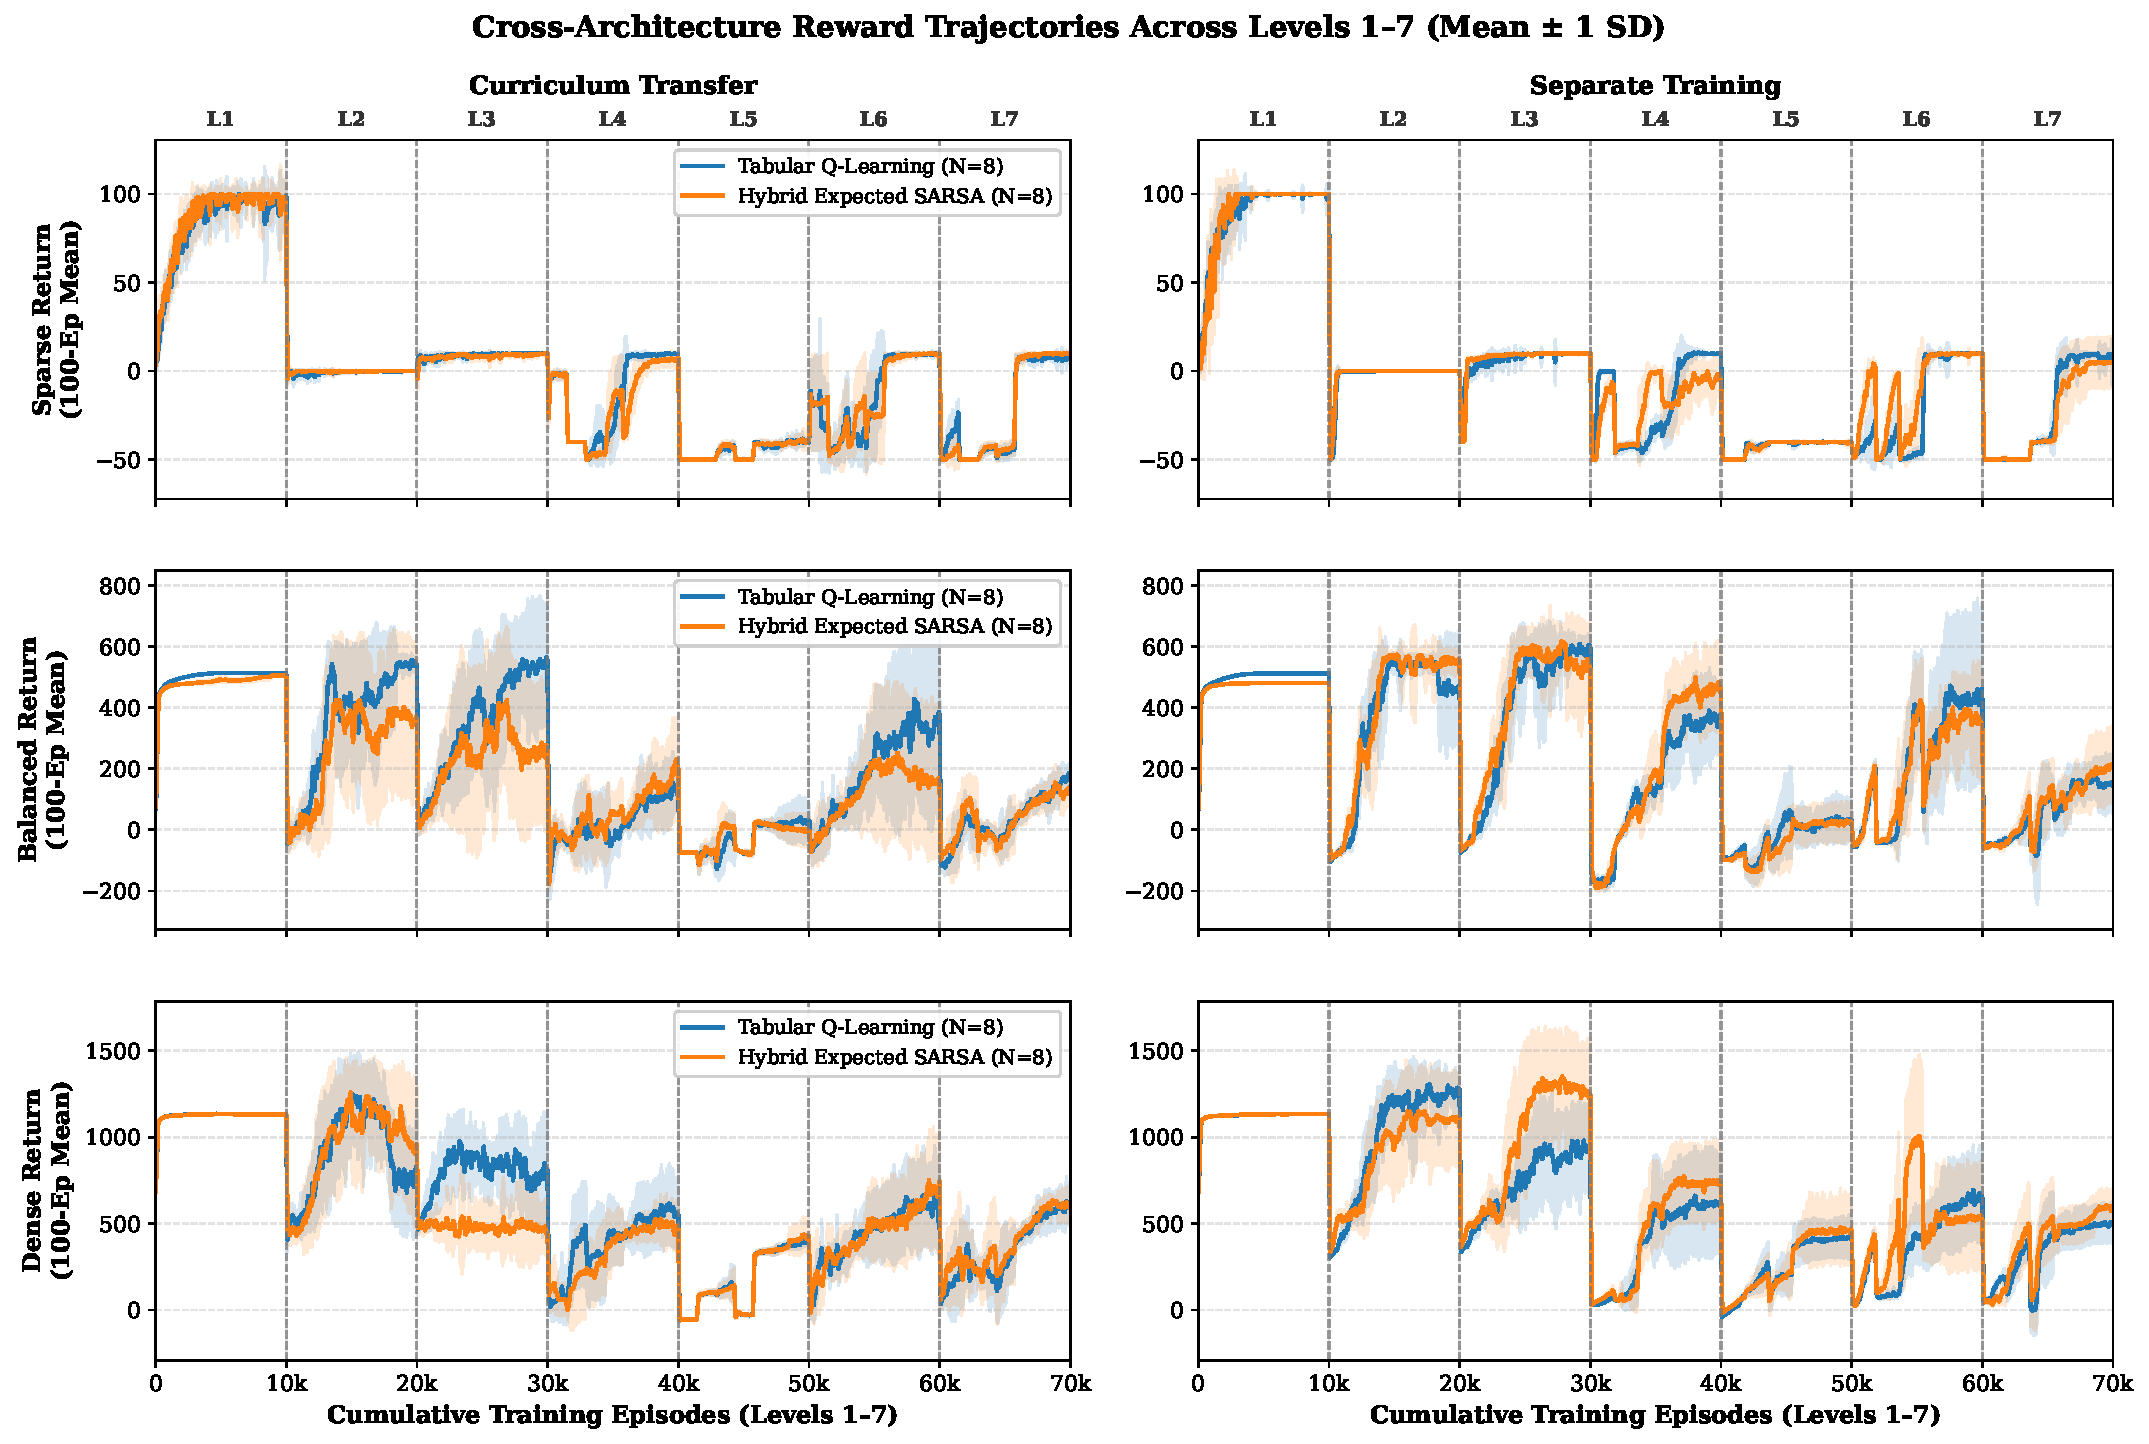
\includegraphics[width=\textwidth]{figures/fig1_reward_trajectories.pdf}
\caption{100-episode rolling reward trajectories (mean $\pm$ 1 SD across 8 seeds) for Sparse (top), Balanced (middle), and Dense (bottom) rewards under Curriculum (left) and Separate (right) training across Levels~1--7.}
\label{fig:reward_trajectories}
\end{figure}

Comparing the three reward settings shows a clear pattern:
\begin{itemize}
    \item \textbf{Sparse fails after Level~1.} On Level~1, agents still reach $87.5\%$--$100.0\%$ Train100 win rates ($50.0\%$--$100.0\%$ Greedy50). From Level~2 to Level~7, every agent and mode ends at $0.0 \pm 0.0\%$. Without step-by-step reward feedback, random exploration rarely finishes a full stage. In Fig.~\ref{fig:reward_trajectories} (top row), Sparse returns on Levels~4--7 briefly rise near $0$--$10$ during reverse-spawn segments close to the goal, but drop back once the spawn shifts to the normal start.
    \item \textbf{Dense encourages rushing and fails on Levels~4--7.} Dense gives $+1.2$ per pixel decrease in goal distance, with a smaller death penalty ($-60.0$) and no hazard-timing penalties. It learns Level~1 ($100.0\%$ Train100) and gets moderate results on Level~2 ($41.8\%$--$86.5\%$ Train100) and Level~3 ($0.0\%$--$60.8\%$), though usually worse than Balanced. On Levels~4--7, Dense gets $0.0\%$ on Levels~4, 5, and 7, and at most $1.5\%$ Train100 ($0.0\%$ Greedy50) on Level~6. Even when Dense shows high return curves in Fig.~\ref{fig:reward_trajectories} (around $+500$ to $+1{,}300$), the agent is only collecting forward-movement points before running into hazards.
    \item \textbf{Balanced is the best reward choice.} Balanced wins $100.0\%$ on Level~1, up to $95.4\%$ Train100 ($100.0\%$ Greedy50) on Level~2, and up to $80.5\%$ Train100 ($100.0\%$ Greedy50) on Level~3. It is also the only reward that wins on Level~4 ($19.6\%$ Train100 / $37.5\%$ Greedy50 for Hybrid Separate) and gets solid wins on Level~6 ($30.8\%$ Train100 / $50.0\%$ Greedy50 for Tabular Separate). For this reason, we keep Reward fixed to \textbf{Balanced} in Sections~\ref{subsec:curr_vs_sep}--\ref{subsec:failures}.
\end{itemize}

\subsection{Curriculum vs.\ Separate \& Agent Comparison}
\label{subsec:curr_vs_sep}

With Reward fixed to \textbf{Balanced}, Fig.~\ref{fig:balanced_overview} shows the full 7-level rolling win-rate curves for both agents and training modes, and Fig.~\ref{fig:spotlight_l3_l4_l6} zooms in on Levels~3, 4, and 6.

\begin{figure}[t]
\centering
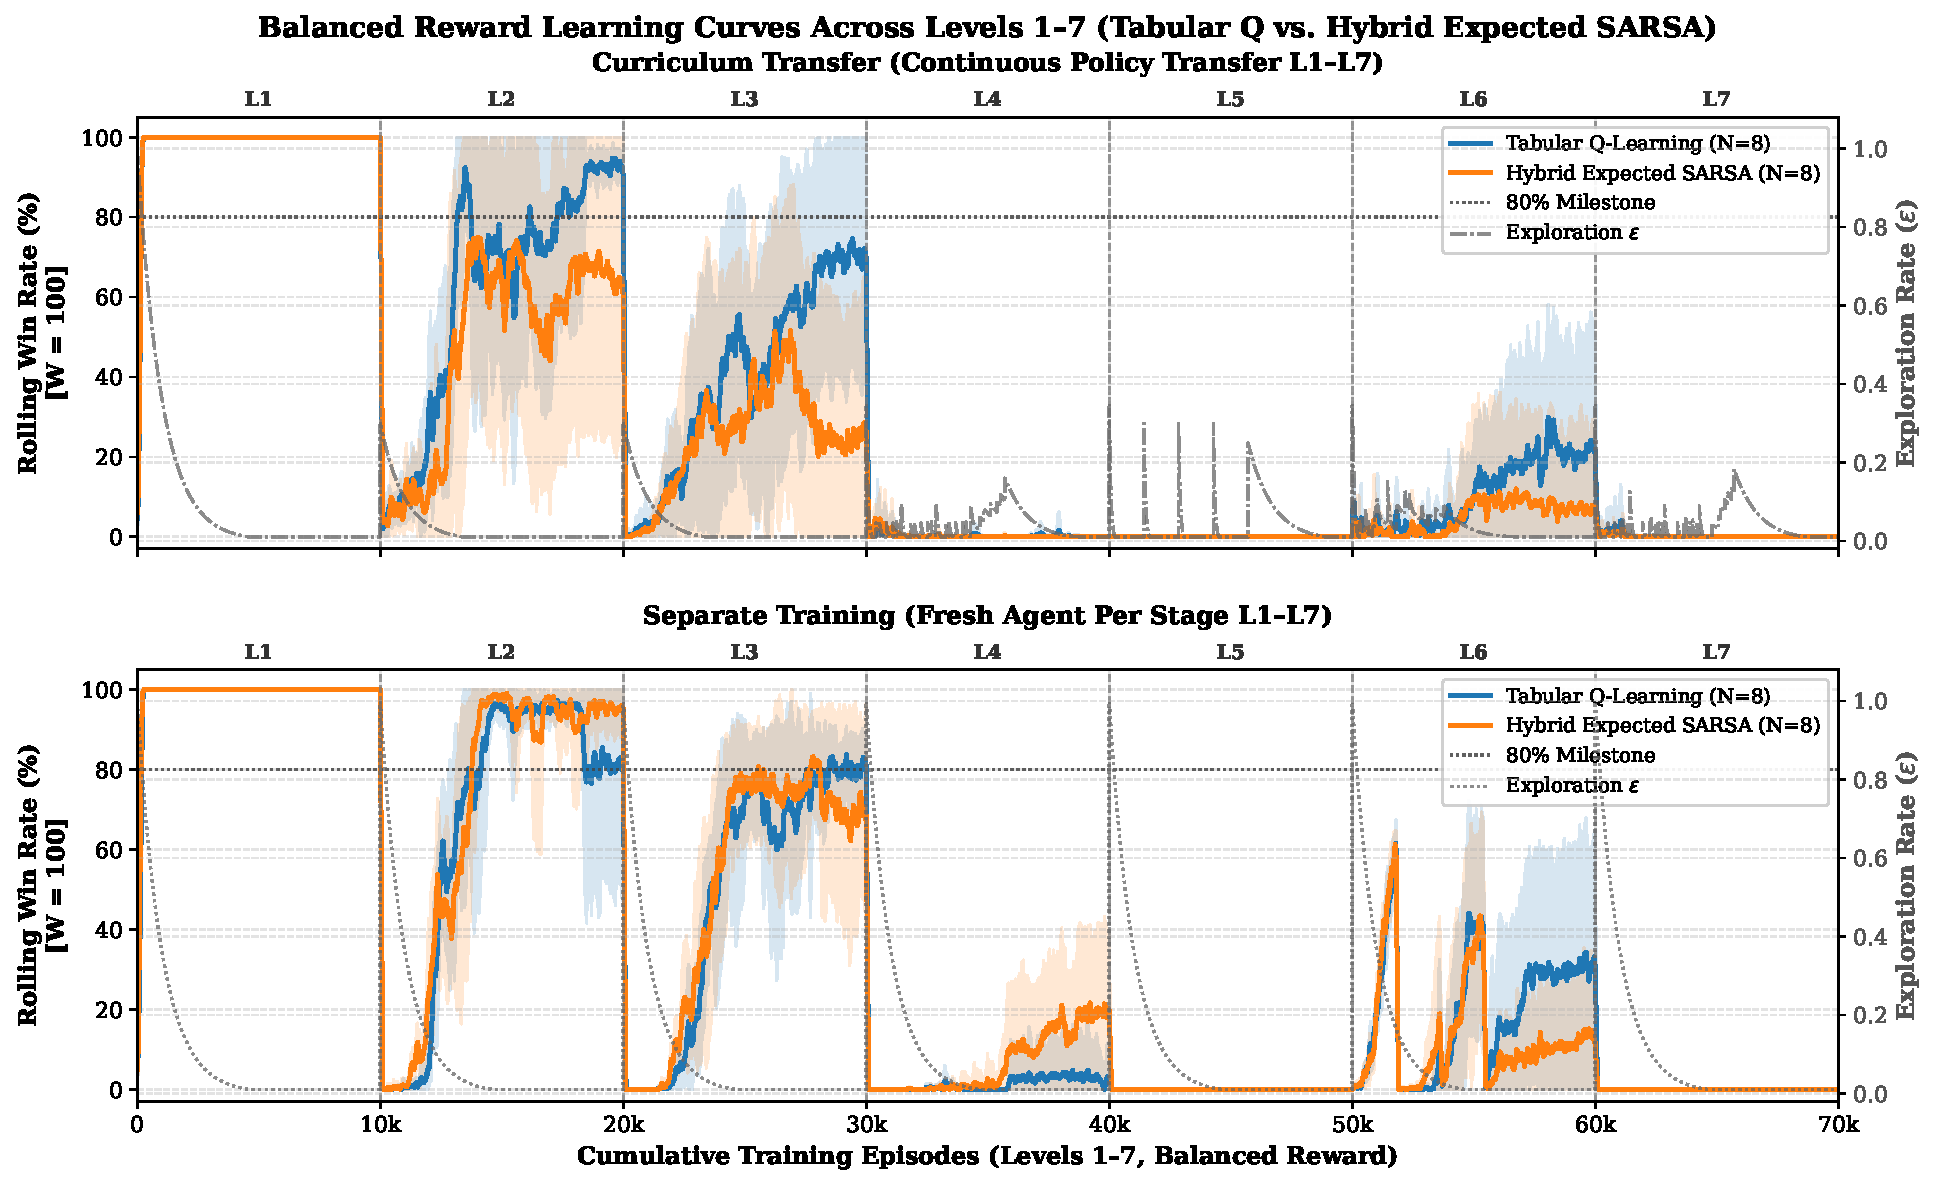
\includegraphics[width=\textwidth]{figures/fig2_balanced_overview.pdf}
\caption{Balanced-reward 100-episode rolling win rate (mean $\pm$ 1 SD) and exploration rate $\epsilon$ across Levels~1--7 for Curriculum Transfer (top) and Separate Training (bottom).}
\label{fig:balanced_overview}
\end{figure}

\begin{figure}[t]
\centering
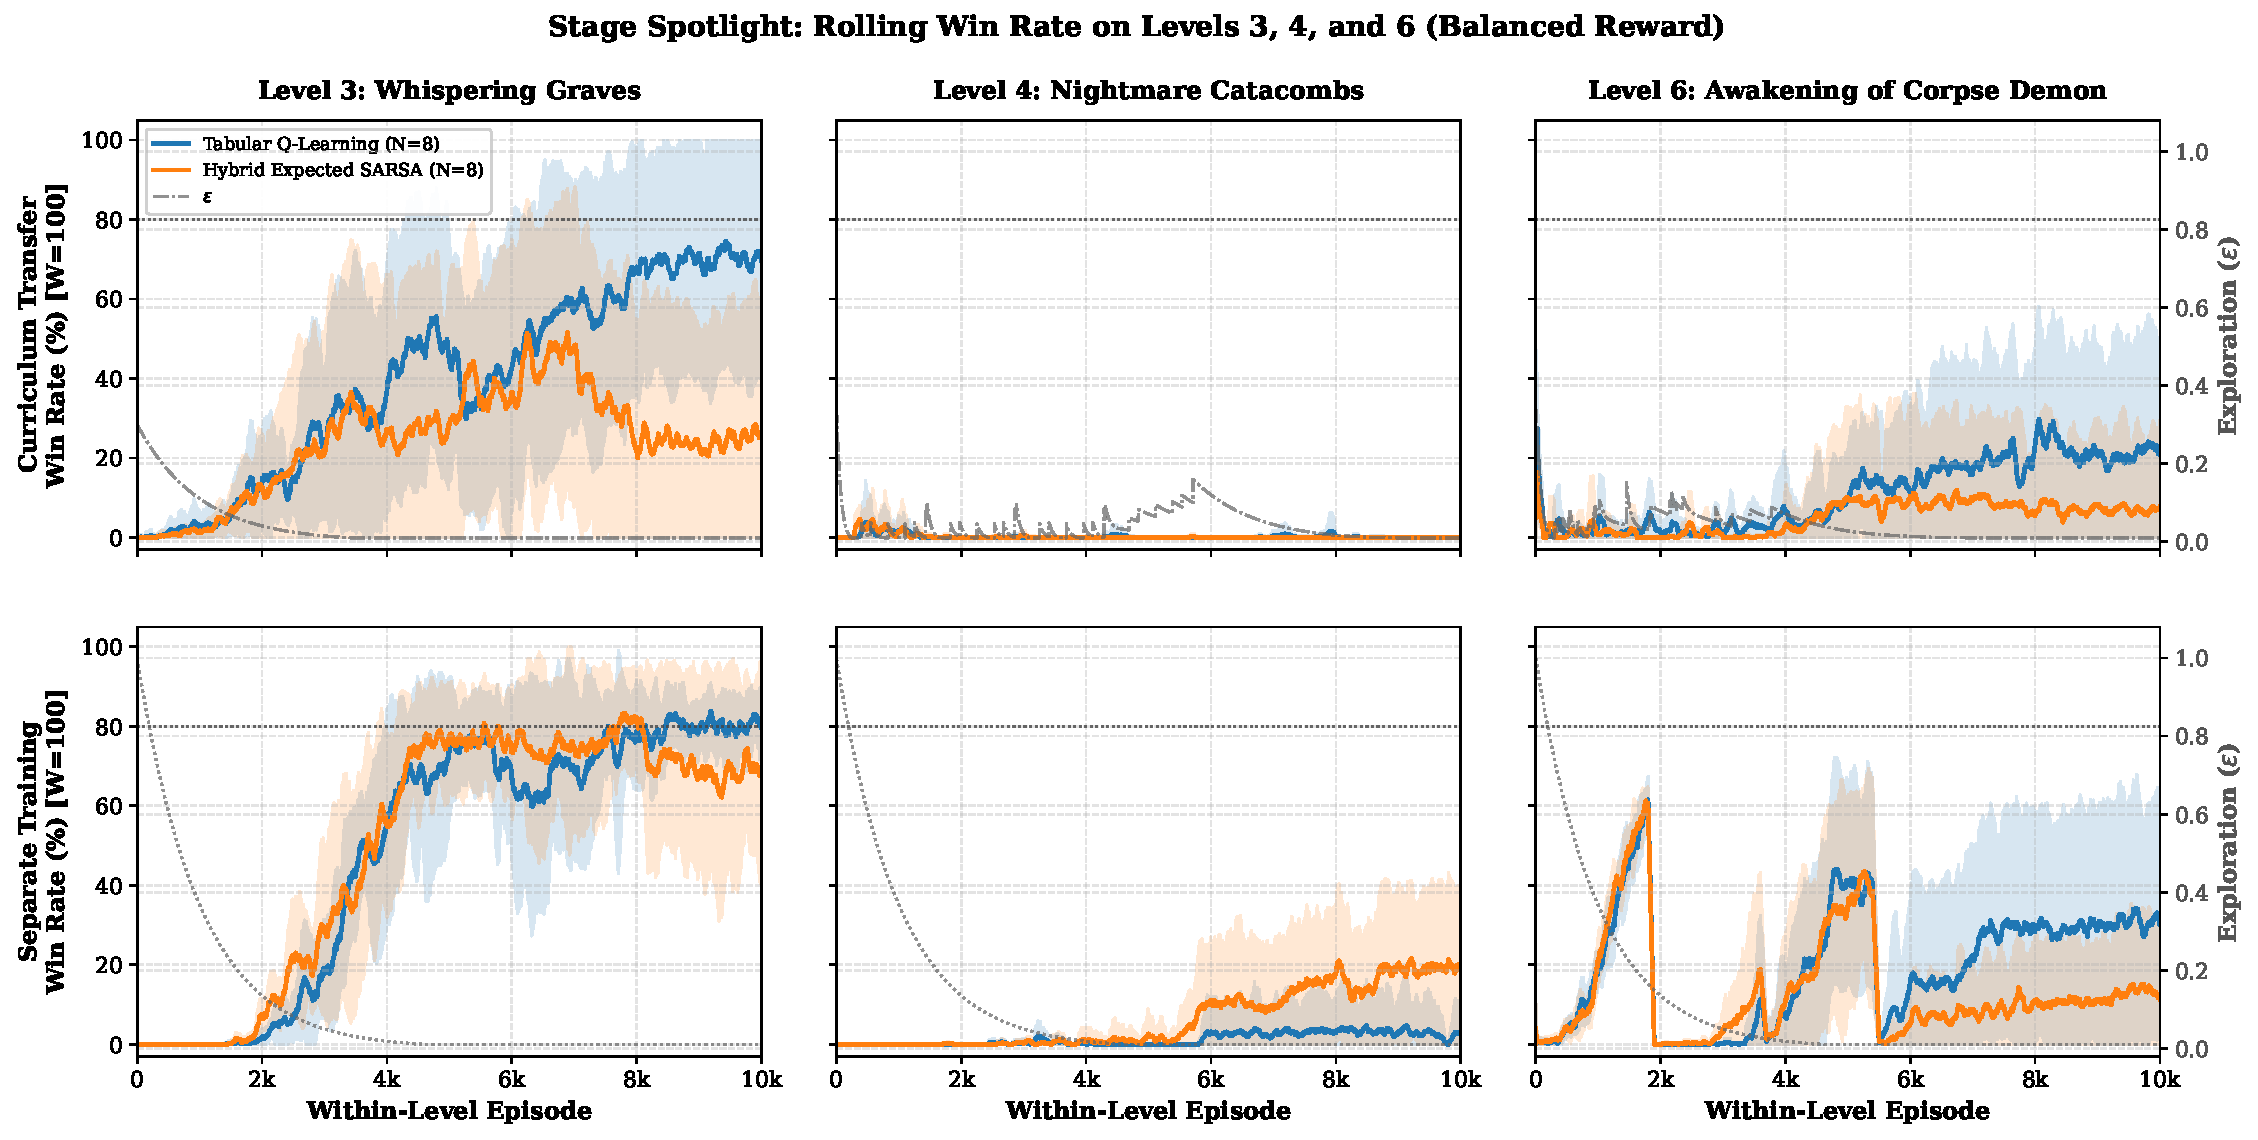
\includegraphics[width=\textwidth]{figures/fig3_spotlight_l3_l4_l6.pdf}
\caption{Within-level rolling win rate on Levels~3, 4, and 6 under Balanced reward for Curriculum Transfer (top) and Separate Training (bottom).}
\label{fig:spotlight_l3_l4_l6}
\end{figure}

Across the two agents, neither wins everywhere. Both reach $100.0 \pm 0.0\%$ on Level~1. On Level~2, Tabular beats Hybrid in Curriculum ($90.8 \pm 5.5\%$ vs.\ $60.6 \pm 41.7\%$ Train100; $100.0\%$ vs.\ $62.5\%$ Greedy50), while Hybrid beats Tabular in Separate ($95.4 \pm 5.4\%$ vs.\ $82.1 \pm 26.9\%$ Train100; $100.0\%$ vs.\ $75.0\%$ Greedy50). On Level~3 and Level~6, Tabular outperforms Hybrid in both modes: on Level~3, Tabular reaches $69.6\%$ (Curriculum) and $80.5\%$ (Separate) vs.\ $26.0\%$ and $67.6\%$ for Hybrid; on Level~6, Tabular reaches $21.2\%$ (Curriculum) and $30.8\%$ (Separate) vs.\ $7.8\%$ and $11.2\%$ for Hybrid. On Level~4, however, Hybrid Separate outperforms Tabular Separate ($19.6 \pm 19.0\%$ vs.\ $2.9 \pm 8.1\%$ Train100; $37.5\%$ vs.\ $12.5\%$ Greedy50) because Expected SARSA lowers the value of states where random exploratory steps near moving hazards can kill the agent.

One surprising result is that \textbf{Separate training beats Curriculum transfer on Levels~3, 4, and 6}:
\begin{itemize}
    \item \textbf{Level~3}: Tabular Separate gets $80.5\%$ Train100 ($100.0\%$ Greedy50) vs.\ $69.6\%$ ($75.0\%$) for Tabular Curriculum; Hybrid Separate gets $67.6\%$ ($87.5\%$) vs.\ $26.0\%$ ($25.0\%$) for Hybrid Curriculum. In Fig.~\ref{fig:spotlight_l3_l4_l6} (left column), Curriculum starts climbing earlier because it already knows basic jumping from Levels~1--2, but Separate starts from $\epsilon = 1.0$, explores more broadly, and settles at a higher win rate with lower variance across seeds.
    \item \textbf{Level~4}: Both Curriculum agents end at $0.0 \pm 0.0\%$, while Separate reaches $19.6\%$ (Hybrid) and $2.9\%$ (Tabular) Train100. In Curriculum mode, $\epsilon$ only re-warms to $0.35$ (and decays quickly at $0.985$ during reverse spawns), while the $50\%$ round-robin replay of Levels~1--3 keeps pulling shared Q-values back toward simpler levels that lack dynamic hazards.
    \item \textbf{Level~6}: Tabular Separate gets $30.8\%$ Train100 ($50.0\%$ Greedy50) vs.\ $21.2\%$ ($25.0\%$) in Curriculum, and Hybrid Separate gets $11.2\%$ vs.\ $7.8\%$ in Curriculum.
\end{itemize}

On Level~6 Separate (Fig.~\ref{fig:spotlight_l3_l4_l6}, bottom right), both agents show two sharp drops around episodes $1{,}800$ ($1.8\text{k}$) and $5{,}400$ ($5.4\text{k}$). This comes directly from the fixed reverse-spawn schedule in \texttt{training/trainer.py}. For episodes $1$--$1{,}800$ ($\le 18\%$ of $10{,}000$), the agent spawns at $0.75$ of the goal distance, so it quickly learns the short final section and reaches about $60\%$ rolling win rate. At episode $1{,}801$, the spawn jumps back to $0.50$ of the goal distance while $\epsilon$ has already decayed to about $0.165$, causing an immediate drop to $0\%$. The agents recover through the $0.50$ and $0.25$ blocks (with a smaller dip around $3.6\text{k}$), climbing above $40\%$ before episode $5{,}400$. At episode $5{,}401$, the spawn switches to the true level start. By then $\epsilon$ has already reached its $0.01$ floor, and because Separate mode does not re-warm $\epsilon$ on spawn shifts, the win rate drops sharply again before slowly recovering to $30.8\%$ (Tabular) and $11.2\%$ (Hybrid).

\subsection{Sample Efficiency}
\label{subsec:sample_efficiency}

Holding Reward fixed to \textbf{Balanced}, Table~\ref{tab:sample_efficiency} and Fig.~\ref{fig:sample_efficiency} compare how fast the agents reach an $80.0\%$ 100-episode rolling win rate and how many simulator steps they spend across Levels~1--7. We separate \textit{Adaptation Steps} (steps inside the current level up to $80\%$ WR), \textit{Pre-Training Steps} (steps spent on earlier levels in Curriculum mode), \textit{Global Steps} (Pre-Training + Adaptation for converging seeds), and \textit{Total Stage Steps} (all steps across the full $10{,}000$-episode stage).

\begin{table}[t]
\caption{Sample efficiency and compute cost (Balanced reward, Levels~1--7). Ep to 80\% WR, Adaptation, Pre-Training, and Global Steps average over the $k/8$ converging seeds; Total Stage Steps averages over all 8 seeds. DNC = Did Not Converge.}
\label{tab:sample_efficiency}
\centering
\resizebox{\textwidth}{!}{%
\begin{tabular}{llcccccc}
\toprule
\textbf{Level} & \textbf{Agent \& Mode} & \textbf{Conv. ($k/N$)} & \textbf{Ep to 80\% WR} & \textbf{Adaptation Steps} & \textbf{Pre-Training Steps} & \textbf{Global Steps to 80\% WR} & \textbf{Total Stage Steps} \\
\midrule
Level 1 & Tabular Curriculum & 8/8 & 165.8 $\pm$ 8.6 & 122,356 $\pm$ 5,963 & 0 $\pm$ 0 & 122,356 $\pm$ 5,963 & 2,050,584 $\pm$ 19,218 \\
Level 1 & Tabular Separate & 8/8 & 176.6 $\pm$ 7.5 & 131,197 $\pm$ 5,302 & 0 & 131,197 $\pm$ 5,302 & 2,163,960 $\pm$ 14,177 \\
Level 1 & Hybrid Expected Curriculum & 8/8 & 160.9 $\pm$ 7.9 & 118,493 $\pm$ 5,660 & 0 $\pm$ 0 & 118,493 $\pm$ 5,660 & 2,348,493 $\pm$ 53,081 \\
Level 1 & Hybrid Expected Separate & 8/8 & 156.5 $\pm$ 8.9 & 115,373 $\pm$ 6,380 & 0 & 115,373 $\pm$ 6,380 & 2,398,197 $\pm$ 3,466 \\
\midrule
Level 2 & Tabular Curriculum & 8/8 & 3,039.9 $\pm$ 284.1 & 630,189 $\pm$ 73,589 & 2,050,584 $\pm$ 19,218 & 2,680,773 $\pm$ 68,334 & 2,383,546 $\pm$ 76,340 \\
Level 2 & Tabular Separate & 8/8 & 3,262.6 $\pm$ 456.8 & 900,836 $\pm$ 137,296 & 0 & 900,836 $\pm$ 137,296 & 2,917,696 $\pm$ 105,929 \\
Level 2 & Hybrid Expected Curriculum & 8/8 & 3,595.8 $\pm$ 1,332.6 & 746,716 $\pm$ 154,209 & 2,348,493 $\pm$ 53,081 & 3,095,208 $\pm$ 167,652 & 2,412,382 $\pm$ 208,318 \\
Level 2 & Hybrid Expected Separate & 8/8 & 3,410.5 $\pm$ 585.3 & 970,581 $\pm$ 190,875 & 0 & 970,581 $\pm$ 190,875 & 2,912,790 $\pm$ 146,503 \\
\midrule
Level 3 & Tabular Curriculum & 7/8 & 5,250.1 $\pm$ 2,246.9 & 1,331,804 $\pm$ 515,862 & 4,431,503 $\pm$ 80,938 & 5,763,307 $\pm$ 540,010 & 2,829,690 $\pm$ 338,387 \\
Level 3 & Tabular Separate & 8/8 & 4,675.1 $\pm$ 917.9 & 1,517,500 $\pm$ 429,207 & 0 & 1,517,500 $\pm$ 429,207 & 3,382,402 $\pm$ 278,286 \\
Level 3 & Hybrid Expected Curriculum & 4/8 & 4,683.5 $\pm$ 2,153.7 & 1,137,576 $\pm$ 369,924 & 4,679,752 $\pm$ 251,585 & 5,817,328 $\pm$ 467,288 & 2,671,212 $\pm$ 387,524 \\
Level 3 & Hybrid Expected Separate & 7/8 & 4,410.0 $\pm$ 807.7 & 1,275,779 $\pm$ 336,151 & 0 & 1,275,779 $\pm$ 336,151 & 3,263,836 $\pm$ 283,039 \\
\midrule
Level 4 & Tabular Curriculum & 0/8 & DNC & DNC & DNC & DNC & 2,688,631 $\pm$ 514,390 \\
Level 4 & Tabular Separate & 0/8 & DNC & DNC & 0 & DNC & 2,533,682 $\pm$ 190,026 \\
Level 4 & Hybrid Expected Curriculum & 0/8 & DNC & DNC & DNC & DNC & 2,157,214 $\pm$ 476,690 \\
Level 4 & Hybrid Expected Separate & 0/8 & DNC & DNC & 0 & DNC & 2,563,432 $\pm$ 221,571 \\
\midrule
Level 5 & Tabular Curriculum & 0/8 & DNC & DNC & DNC & DNC & 822,320 $\pm$ 62,509 \\
Level 5 & Tabular Separate & 0/8 & DNC & DNC & 0 & DNC & 1,084,920 $\pm$ 228,581 \\
Level 5 & Hybrid Expected Curriculum & 0/8 & DNC & DNC & DNC & DNC & 853,636 $\pm$ 82,909 \\
Level 5 & Hybrid Expected Separate & 0/8 & DNC & DNC & 0 & DNC & 909,847 $\pm$ 104,445 \\
\midrule
Level 6 & Tabular Curriculum & 1/8 & 6,388.0 & 1,366,889 & 9,419,566 & 10,786,455 & 2,339,462 $\pm$ 697,104 \\
Level 6 & Tabular Separate & 2/8 & 7,043.0 $\pm$ 3,245.6 & 1,473,665 $\pm$ 1,137,251 & 0 & 1,473,665 $\pm$ 1,137,251 & 2,332,832 $\pm$ 501,266 \\
Level 6 & Hybrid Expected Curriculum & 0/8 & DNC & DNC & DNC & DNC & 2,133,405 $\pm$ 612,632 \\
Level 6 & Hybrid Expected Separate & 0/8 & DNC & DNC & 0 & DNC & 2,143,057 $\pm$ 335,087 \\
\midrule
Level 7 & Tabular Curriculum & 0/8 & DNC & DNC & DNC & DNC & 1,789,969 $\pm$ 150,160 \\
Level 7 & Tabular Separate & 0/8 & DNC & DNC & 0 & DNC & 1,670,050 $\pm$ 332,654 \\
Level 7 & Hybrid Expected Curriculum & 0/8 & DNC & DNC & DNC & DNC & 1,770,178 $\pm$ 152,428 \\
Level 7 & Hybrid Expected Separate & 0/8 & DNC & DNC & 0 & DNC & 1,680,126 $\pm$ 272,547 \\
\bottomrule
\end{tabular}%
}
\end{table}

\begin{figure}[t]
\centering
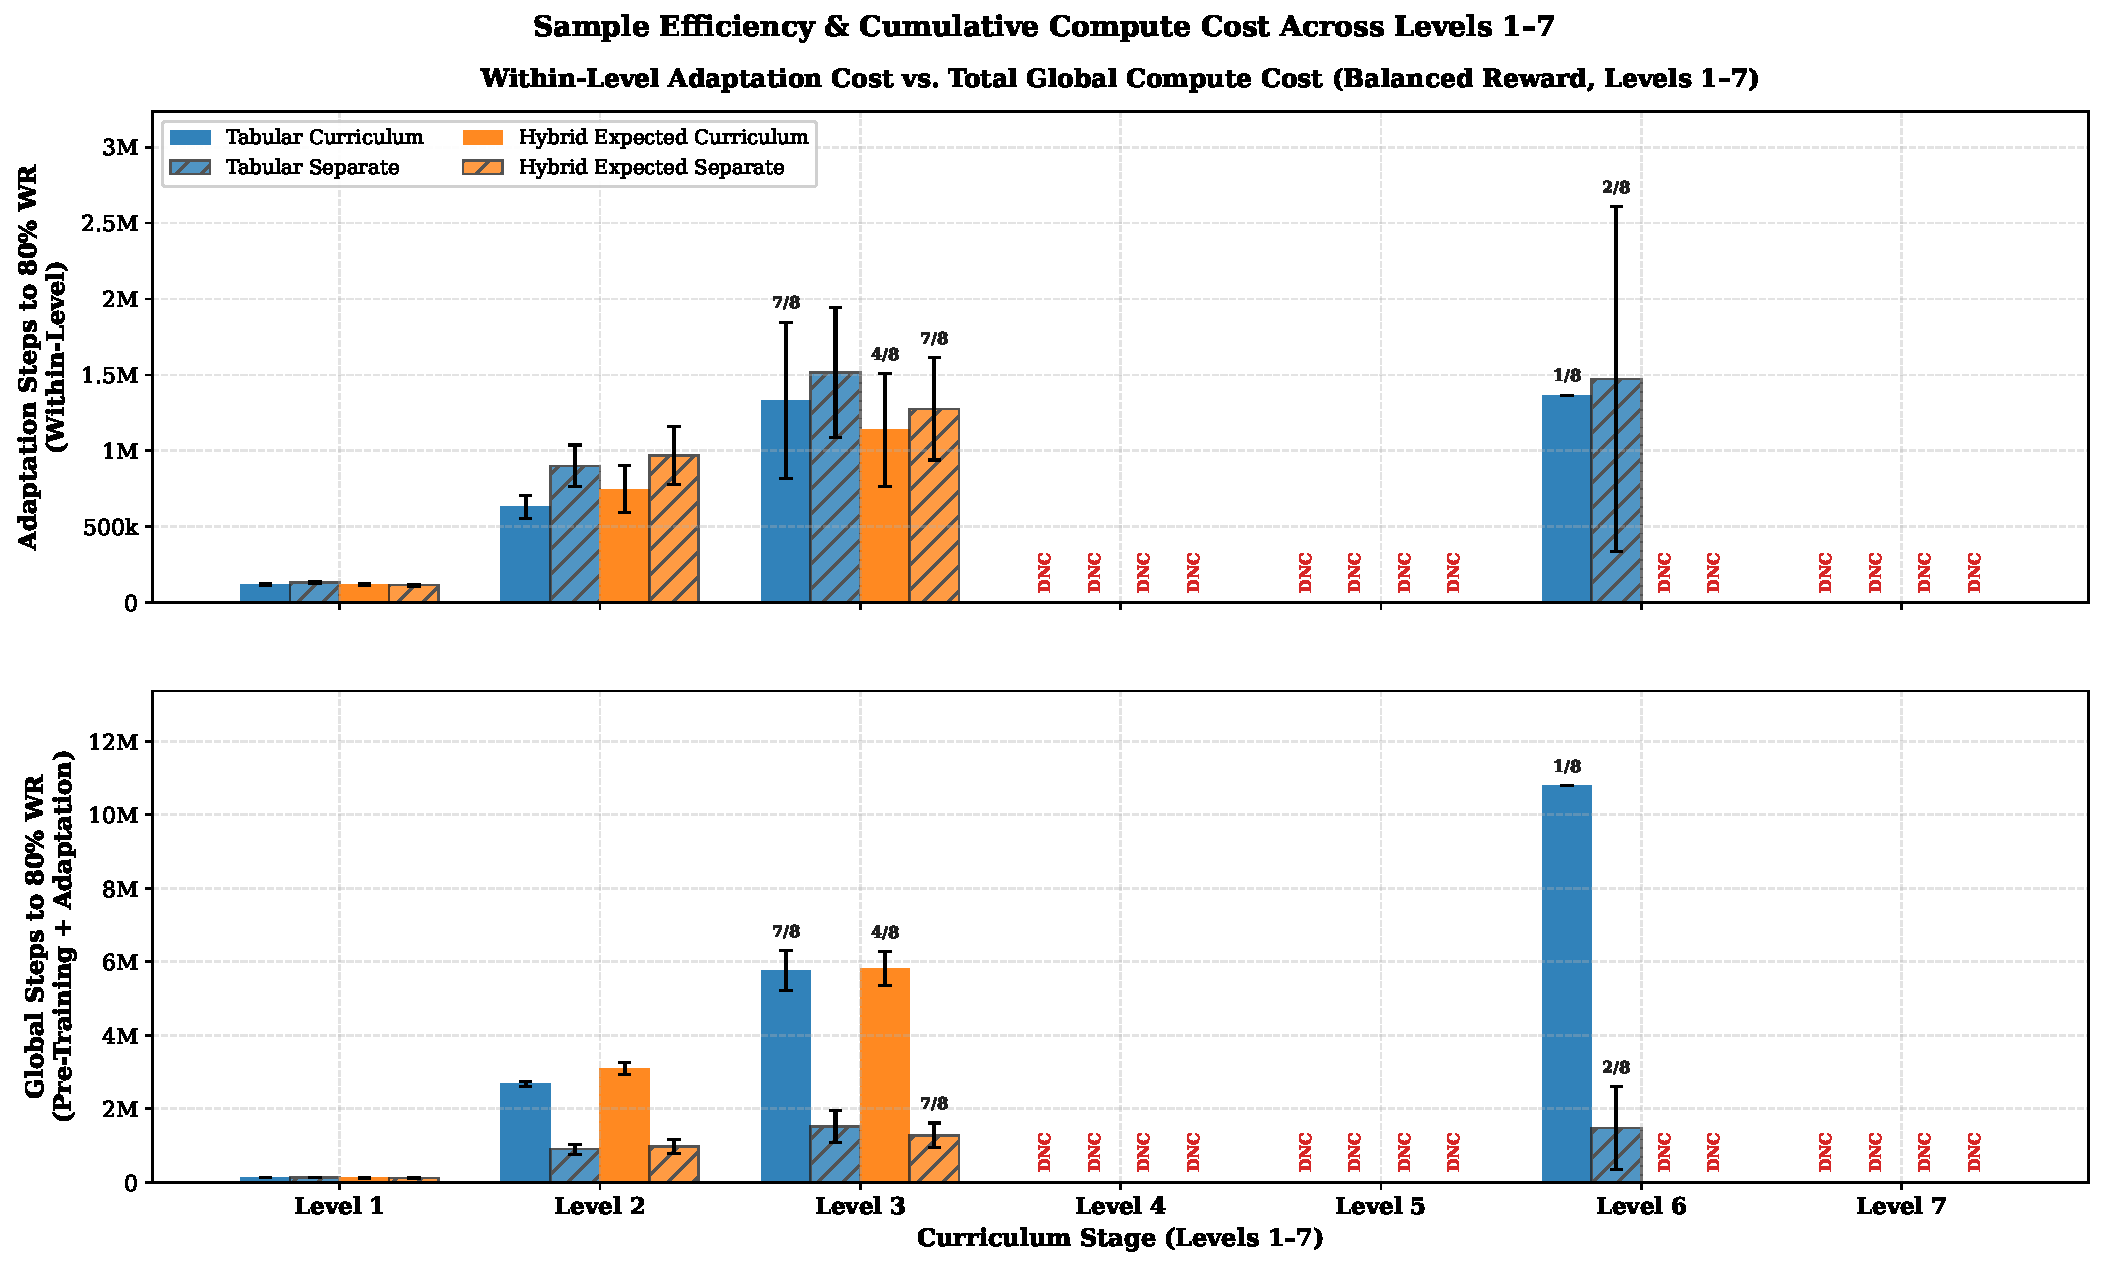
\includegraphics[width=\textwidth]{figures/fig4_sample_efficiency.pdf}
\caption{Within-level adaptation steps (top) and global compute steps (bottom) to reach an $80\%$ rolling win rate under Balanced reward across Levels~1--7.}
\label{fig:sample_efficiency}
\end{figure}

Three points stand out in Table~\ref{tab:sample_efficiency} and Fig.~\ref{fig:sample_efficiency}:
\begin{enumerate}
    \item \textbf{Within-level speed vs.\ global compute.} On Level~1, all four settings converge on $8/8$ seeds in $156.5$--$176.6$ episodes ($115{,}373$--$131{,}197$ steps). On Level~2, all four still converge on $8/8$ seeds, and Curriculum cuts within-level adaptation steps by $30.0\%$ for Tabular ($630{,}189$ vs.\ $900{,}836$) and $23.1\%$ for Hybrid ($746{,}716$ vs.\ $970{,}581$). However, once we add the $2.05\text{M}$--$2.35\text{M}$ pre-training steps from Level~1, Curriculum takes nearly $3\times$ more global steps ($2.68\text{M}$ and $3.10\text{M}$ vs.\ $0.90\text{M}$ and $0.97\text{M}$).
    \item \textbf{Lower convergence rate on Level~3 and Level~6.} On Level~3, Separate reaches $80\%$ WR more reliably ($8/8$ for Tabular, $7/8$ for Hybrid) than Curriculum ($7/8$ for Tabular, $4/8$ for Hybrid), while requiring only $1.28\text{M}$--$1.52\text{M}$ global steps compared to $5.76\text{M}$--$5.82\text{M}$ for Curriculum. On Level~6, only Tabular converges on a few seeds ($2/8$ Separate at $1.47\text{M}$ steps; $1/8$ Curriculum at $10.79\text{M}$ global steps), while Hybrid stays at $0/8$.
    \item \textbf{Total stage steps reflect survival time.} Levels~4, 5, and 7 never hit $80\%$ WR ($0/8$ DNC). Level~5 has the lowest Total Stage Steps ($0.82\text{M}$--$1.08\text{M}$, around $82$--$108$ steps per episode) because agents die early in pits and hazards, whereas Level~1 spends $2.05\text{M}$--$2.40\text{M}$ steps across $10{,}000$ full winning runs.
\end{enumerate}

\subsection{Why Hard Levels Fail \& Limitations}
\label{subsec:failures}

Table~\ref{tab:failure_modes} summarizes the outcome breakdown and discovered state counts on Levels~4--7 under Balanced reward. Note that unlike Table~\ref{tab:overall_winrates} (which reports only the final 100 episodes), the Win \%, Timeout \%, Pit Death \%, and Hazard/Entity Death \% columns in Table~\ref{tab:failure_modes} are averaged across \textbf{all $10{,}000$ training episodes} per stage (including early reverse-spawn episodes). Hazard/Entity Death \% groups all non-pit lethal collisions (ghosts, fire, lasers, wisps, and grave monsters).

\begin{table}[t]
\caption{Failure breakdown and discovered state counts on Levels~4--7 (Balanced reward). Percentages average across all $10{,}000$ training episodes per level across 8 seeds.}
\label{tab:failure_modes}
\centering
\resizebox{\textwidth}{!}{%
\begin{tabular}{llccccc}
\toprule
\textbf{Level} & \textbf{Agent \& Mode} & \textbf{Win \% (All 10k)} & \textbf{Timeout \%} & \textbf{Pit Death \%} & \textbf{Hazard/Entity Death \%} & \textbf{Discovered States} \\
\midrule
Level 4 & Tabular Curriculum & 0.2 $\pm$ 0.2\% & 42.0 $\pm$ 7.2\% & 36.8 $\pm$ 7.1\% & 20.9 $\pm$ 3.5\% & 1,672 $\pm$ 187 \\
Level 4 & Tabular Separate & 1.3 $\pm$ 3.3\% & 52.4 $\pm$ 4.2\% & 25.6 $\pm$ 2.0\% & 20.7 $\pm$ 2.7\% & 1,562 $\pm$ 57 \\
Level 4 & Hybrid Expected Curriculum & 0.2 $\pm$ 0.2\% & 38.7 $\pm$ 7.6\% & 38.7 $\pm$ 10.4\% & 22.4 $\pm$ 5.0\% & 1,690 $\pm$ 103 \\
Level 4 & Hybrid Expected Separate & 6.6 $\pm$ 6.3\% & 47.1 $\pm$ 11.6\% & 19.1 $\pm$ 3.0\% & 27.3 $\pm$ 8.4\% & 1,771 $\pm$ 66 \\
\midrule
Level 5 & Tabular Curriculum & 0.0 $\pm$ 0.0\% & 40.1 $\pm$ 5.3\% & 26.3 $\pm$ 4.9\% & 33.6 $\pm$ 5.9\% & 5,688 $\pm$ 343 \\
Level 5 & Tabular Separate & 0.0 $\pm$ 0.0\% & 26.1 $\pm$ 6.0\% & 46.6 $\pm$ 10.9\% & 27.2 $\pm$ 6.0\% & 4,616 $\pm$ 392 \\
Level 5 & Hybrid Expected Curriculum & 0.0 $\pm$ 0.0\% & 43.2 $\pm$ 5.8\% & 31.8 $\pm$ 6.0\% & 24.9 $\pm$ 6.0\% & 5,718 $\pm$ 188 \\
Level 5 & Hybrid Expected Separate & 0.0 $\pm$ 0.0\% & 22.1 $\pm$ 3.6\% & 48.6 $\pm$ 12.9\% & 29.3 $\pm$ 12.0\% & 4,358 $\pm$ 337 \\
\midrule
Level 6 & Tabular Curriculum & 10.9 $\pm$ 10.8\% & 33.7 $\pm$ 5.0\% & 15.9 $\pm$ 8.2\% & 39.5 $\pm$ 10.3\% & 6,716 $\pm$ 257 \\
Level 6 & Tabular Separate & 19.6 $\pm$ 13.0\% & 33.3 $\pm$ 10.7\% & 8.5 $\pm$ 6.6\% & 38.5 $\pm$ 7.1\% & 2,077 $\pm$ 125 \\
Level 6 & Hybrid Expected Curriculum & 5.0 $\pm$ 11.2\% & 38.0 $\pm$ 5.9\% & 27.7 $\pm$ 14.8\% & 29.2 $\pm$ 9.2\% & 6,726 $\pm$ 186 \\
Level 6 & Hybrid Expected Separate & 13.3 $\pm$ 7.8\% & 33.8 $\pm$ 11.1\% & 12.2 $\pm$ 6.4\% & 40.7 $\pm$ 7.5\% & 1,973 $\pm$ 70 \\
\midrule
Level 7 & Tabular Curriculum & 0.2 $\pm$ 0.3\% & 49.9 $\pm$ 5.6\% & 23.2 $\pm$ 4.5\% & 26.7 $\pm$ 4.5\% & 9,413 $\pm$ 302 \\
Level 7 & Tabular Separate & 0.0 $\pm$ 0.0\% & 53.0 $\pm$ 5.6\% & 26.3 $\pm$ 5.8\% & 20.7 $\pm$ 3.4\% & 4,326 $\pm$ 419 \\
Level 7 & Hybrid Expected Curriculum & 0.1 $\pm$ 0.1\% & 41.5 $\pm$ 6.6\% & 29.2 $\pm$ 6.6\% & 29.1 $\pm$ 4.3\% & 9,130 $\pm$ 194 \\
Level 7 & Hybrid Expected Separate & 0.0 $\pm$ 0.0\% & 50.5 $\pm$ 7.2\% & 28.5 $\pm$ 6.4\% & 20.9 $\pm$ 3.9\% & 4,187 $\pm$ 365 \\
\bottomrule
\end{tabular}%
}
\end{table}

Table~\ref{tab:failure_modes} shows clear failure patterns across the hard stages:
\begin{itemize}
    \item \textbf{Level~4 (Timeouts and pits):} Timeouts are the largest share ($38.7\%$--$52.4\%$), followed by pit deaths ($19.1\%$--$38.7\%$) and hazard deaths ($20.7\%$--$27.3\%$). Separate training cuts pit deaths down to $19.1\%$ (Hybrid) and $25.6\%$ (Tabular), but many runs still stall until timeout in front of moving hazards.
    \item \textbf{Level~5 ($0.0\%$ wins across all 10k episodes):} Separate agents die mostly in pits ($46.6\%$ Tabular, $48.6\%$ Hybrid) and hazards ($27.2\%$--$29.3\%$), while Curriculum agents stall more often ($40.1\%$--$43.2\%$ timeouts).
    \item \textbf{Level~6 (Partial wins, mostly hazard deaths):} Hazard/entity deaths are the main failure ($29.2\%$--$40.7\%$) alongside timeouts ($33.3\%$--$38.0\%$), whereas pit deaths drop to $8.5\%$--$12.2\%$ in Separate mode.
    \item \textbf{Level~7 (Timeouts dominate):} Timeouts account for $41.5\%$--$53.0\%$ of episodes, with $23.2\%$--$29.2\%$ pit deaths and $20.7\%$--$29.1\%$ hazard deaths, leaving near-zero wins ($0.0\%$--$0.2\%$).
\end{itemize}

Four main limitations explain why these failures happen:
\begin{enumerate}
    \item \textbf{15-tuple state space and perceptual aliasing:} In \texttt{discretizer/state\_discretizer.py}, continuous game states are quantized into a 15-tuple (\texttt{grounded}, \texttt{vy}, \texttt{obs\_dist}, \texttt{obs\_height}, \texttt{pit\_dist}, \texttt{ghost\_dist}, \texttt{ghost\_alt}, \texttt{laser}, \texttt{wisp}, \texttt{crouch}, \texttt{double\_jump}, \texttt{monster}, \texttt{pit\_width}, \texttt{ghost\_vx}, \texttt{vx}) with $8{,}847{,}360$ theoretical states. In practice, agents only visit $1{,}562$--$9{,}413$ states (under $0.11\%$). Because each bin tracks only the nearest entity within coarse distance ranges (such as $0$--$80\text{ px}$ or $0$--$100\text{ px}$) without exact timers or multi-entity ordering, different hazard combinations fall into the same discrete state. A tabular Q-table averages those conflicting outcomes, leading either to hesitation (timeouts) or mistimed jumps (pit and hazard deaths).
    \item \textbf{Negative transfer in Curriculum mode:} Curriculum carries Q-values from earlier stages and replays prior levels on $50\%$ of episodes. Look at Table~\ref{tab:failure_modes}: on Level~6, Curriculum uses $6{,}716$--$6{,}726$ cumulative states, while Separate reaches higher win rates using only $1{,}973$--$2{,}077$ states. Replaying simpler stages pulls shared aliased states back toward habits that fail under combined hazards.
    \item \textbf{Exploration schedule on reverse spawns:} In Separate mode, $\epsilon$ decays to $0.01$ around episode $4{,}603$, before the full-level phase starts at episode $5{,}401$, leaving too little exploration for the start of Levels~5--7.
    \item \textbf{Fixed bin thresholds:} Distance and velocity cutoffs are tuned by hand, so changing level timing or adding simultaneous enemies cannot be fixed without a richer model such as a neural network.
\end{enumerate}

\subsection{Checkpoint Blind Evaluation (1,000 Procedural Episodes per Level)}
\label{subsec:checkpoint_eval}

To test how well the trained policies work on unseen layouts, we take each saved best per-level checkpoint (\texttt{q\_table\_lvl\{1..7\}\_best.pkl}) and run a blind greedy test ($\epsilon = 0.0$) over $1{,}000$ procedural maps generated by \texttt{LevelGenerator} (map seeds $1$--$1{,}000$) in \texttt{evaluation/eval\_checkpoints\_1000.py}. Table~\ref{tab:checkpoint_blind} reports the mean $\pm$ SD win rate and episode reward across the $8$ training seeds ($42$--$49$) for all $7$ levels, $2$ agents, $2$ modes, and $3$ rewards.

\begin{table}[t]
\caption{Blind greedy evaluation over $1{,}000$ procedural map seeds per level (mean $\pm$ SD across 8 training seeds). Values show Win Rate (\%) / Mean Episode Reward.}
\label{tab:checkpoint_blind}
\centering
\resizebox{\textwidth}{!}{%
\begin{tabular}{llcccc}
\toprule
\textbf{Level} & \textbf{Reward} & \textbf{Tabular Curr} & \textbf{Hybrid Curr} & \textbf{Tabular Sep} & \textbf{Hybrid Sep} \\
 & & \textbf{(WR \% / Reward)} & \textbf{(WR \% / Reward)} & \textbf{(WR \% / Reward)} & \textbf{(WR \% / Reward)} \\
\midrule
Level 1 & Balanced & 97.1 $\pm$ 8.1\% / 696.2 $\pm$ 100.7 & 100.0 $\pm$ 0.0\% / 722.3 $\pm$ 5.0 & 100.0 $\pm$ 0.0\% / 728.5 $\pm$ 3.1 & 98.7 $\pm$ 3.7\% / 670.8 $\pm$ 126.5 \\
Level 1 & Dense & 93.1 $\pm$ 19.4\% / 1,771.2 $\pm$ 196.3 & 100.0 $\pm$ 0.0\% / 1,841.5 $\pm$ 1.5 & 90.1 $\pm$ 23.1\% / 1,749.6 $\pm$ 208.6 & 95.7 $\pm$ 12.1\% / 1,745.6 $\pm$ 261.0 \\
Level 1 & Sparse & 100.0 $\pm$ 0.1\% / 100.0 $\pm$ 0.1 & 90.4 $\pm$ 27.0\% / 90.4 $\pm$ 27.0 & 78.2 $\pm$ 37.3\% / 78.2 $\pm$ 37.3 & 66.0 $\pm$ 38.4\% / 66.0 $\pm$ 38.4 \\
\midrule
Level 2 & Balanced & 1.4 $\pm$ 0.7\% / -316.8 $\pm$ 954.1 & 1.5 $\pm$ 1.6\% / -174.5 $\pm$ 401.9 & 1.7 $\pm$ 1.5\% / 13.0 $\pm$ 55.1 & 3.1 $\pm$ 1.2\% / 45.4 $\pm$ 19.8 \\
Level 2 & Dense & 1.6 $\pm$ 1.2\% / 570.5 $\pm$ 146.0 & 1.1 $\pm$ 1.2\% / 571.1 $\pm$ 89.6 & 1.5 $\pm$ 0.9\% / 618.4 $\pm$ 46.1 & 1.4 $\pm$ 0.6\% / 598.8 $\pm$ 51.6 \\
Level 2 & Sparse & 0.0 $\pm$ 0.0\% / -29.7 $\pm$ 17.2 & 0.0 $\pm$ 0.0\% / -32.6 $\pm$ 13.8 & 0.0 $\pm$ 0.0\% / -44.9 $\pm$ 0.5 & 0.0 $\pm$ 0.0\% / -0.6 $\pm$ 1.7 \\
\midrule
Level 3 & Balanced & 1.7 $\pm$ 1.6\% / 82.2 $\pm$ 52.6 & 2.2 $\pm$ 3.1\% / 75.0 $\pm$ 97.4 & 0.5 $\pm$ 0.2\% / -28.7 $\pm$ 57.5 & 0.8 $\pm$ 0.2\% / 22.0 $\pm$ 4.9 \\
Level 3 & Dense & 0.8 $\pm$ 0.9\% / 596.5 $\pm$ 72.6 & 0.5 $\pm$ 0.8\% / 561.5 $\pm$ 81.1 & 0.1 $\pm$ 0.2\% / 405.8 $\pm$ 42.3 & 0.2 $\pm$ 0.2\% / 442.3 $\pm$ 36.2 \\
Level 3 & Sparse & 0.0 $\pm$ 0.0\% / -29.3 $\pm$ 17.0 & 0.0 $\pm$ 0.0\% / -38.3 $\pm$ 11.0 & 0.0 $\pm$ 0.0\% / -44.3 $\pm$ 0.4 & 0.0 $\pm$ 0.0\% / -41.8 $\pm$ 5.7 \\
\midrule
Level 4 & Balanced & 0.2 $\pm$ 0.2\% / 70.7 $\pm$ 112.9 & 0.3 $\pm$ 0.3\% / 66.8 $\pm$ 121.7 & 0.6 $\pm$ 0.4\% / 142.8 $\pm$ 29.4 & 0.5 $\pm$ 0.4\% / 139.2 $\pm$ 55.6 \\
Level 4 & Dense & 0.1 $\pm$ 0.1\% / 517.0 $\pm$ 70.6 & 0.0 $\pm$ 0.0\% / 496.5 $\pm$ 87.2 & 0.0 $\pm$ 0.0\% / 513.4 $\pm$ 93.1 & 0.0 $\pm$ 0.0\% / 506.1 $\pm$ 38.6 \\
Level 4 & Sparse & 0.0 $\pm$ 0.0\% / -4.4 $\pm$ 5.5 & 0.0 $\pm$ 0.0\% / -5.8 $\pm$ 6.4 & 0.0 $\pm$ 0.0\% / -12.7 $\pm$ 9.9 & 0.0 $\pm$ 0.0\% / -4.4 $\pm$ 9.6 \\
\midrule
Level 5 & Balanced & 0.0 $\pm$ 0.0\% / -8.1 $\pm$ 93.8 & 0.0 $\pm$ 0.0\% / 27.5 $\pm$ 6.6 & 0.0 $\pm$ 0.0\% / 39.2 $\pm$ 8.4 & 0.0 $\pm$ 0.0\% / 27.3 $\pm$ 13.4 \\
Level 5 & Dense & 0.0 $\pm$ 0.0\% / 391.1 $\pm$ 17.4 & 0.0 $\pm$ 0.0\% / 401.5 $\pm$ 15.3 & 0.0 $\pm$ 0.0\% / 410.1 $\pm$ 13.0 & 0.0 $\pm$ 0.0\% / 424.1 $\pm$ 26.6 \\
Level 5 & Sparse & 0.0 $\pm$ 0.0\% / -36.7 $\pm$ 13.2 & 0.0 $\pm$ 0.0\% / -43.0 $\pm$ 1.2 & 0.0 $\pm$ 0.0\% / -36.9 $\pm$ 15.6 & 0.0 $\pm$ 0.0\% / -44.3 $\pm$ 0.2 \\
\midrule
Level 6 & Balanced & 0.5 $\pm$ 0.4\% / 70.6 $\pm$ 23.8 & 0.7 $\pm$ 0.6\% / 92.8 $\pm$ 12.8 & 0.1 $\pm$ 0.1\% / 14.8 $\pm$ 17.4 & 0.1 $\pm$ 0.1\% / 18.5 $\pm$ 21.0 \\
Level 6 & Dense & 0.1 $\pm$ 0.2\% / 427.3 $\pm$ 40.2 & 0.0 $\pm$ 0.1\% / 420.5 $\pm$ 25.8 & 0.0 $\pm$ 0.0\% / 358.1 $\pm$ 34.7 & 0.0 $\pm$ 0.0\% / 352.8 $\pm$ 19.5 \\
Level 6 & Sparse & 0.0 $\pm$ 0.0\% / -28.6 $\pm$ 9.6 & 0.0 $\pm$ 0.0\% / -33.6 $\pm$ 6.5 & 0.0 $\pm$ 0.0\% / -35.5 $\pm$ 9.5 & 0.0 $\pm$ 0.0\% / -25.5 $\pm$ 10.3 \\
\midrule
Level 7 & Balanced & 0.0 $\pm$ 0.0\% / 21.3 $\pm$ 66.2 & 0.0 $\pm$ 0.0\% / 47.5 $\pm$ 14.7 & 0.0 $\pm$ 0.0\% / -11.1 $\pm$ 25.2 & 0.0 $\pm$ 0.0\% / 1.4 $\pm$ 27.1 \\
Level 7 & Dense & 0.0 $\pm$ 0.0\% / 359.7 $\pm$ 49.1 & 0.0 $\pm$ 0.0\% / 388.4 $\pm$ 25.7 & 0.0 $\pm$ 0.0\% / 296.0 $\pm$ 37.3 & 0.0 $\pm$ 0.0\% / 300.5 $\pm$ 33.6 \\
Level 7 & Sparse & 0.0 $\pm$ 0.0\% / -34.7 $\pm$ 7.7 & 0.0 $\pm$ 0.0\% / -42.7 $\pm$ 6.7 & 0.0 $\pm$ 0.0\% / -37.8 $\pm$ 11.0 & 0.0 $\pm$ 0.0\% / -34.0 $\pm$ 9.3 \\
\bottomrule
\end{tabular}%
}
\end{table}

Table~\ref{tab:checkpoint_blind} shows a sharp split between Level~1 and Levels~2--7:
\begin{itemize}
    \item \textbf{Level~1 transfers well to new maps ($66.0\%$--$100.0\%$).} Balanced achieves $97.1\%$--$100.0\%$ and Dense reaches $90.1\%$--$100.0\%$, while Sparse gets $66.0\%$--$100.0\%$. Comparing \texttt{env/map\_levels.py} and \texttt{env/level\_generator.py} explains why: both the fixed and procedural Level~1 maps have only static tombstones on flat ground, with no pits or moving hazards. Because the discretizer tracks local obstacle distance and height relative to the player, the jump timing learned on the fixed map works across procedural Level~1 maps ($1{,}300$--$1{,}700\text{ px}$ long, tombstone heights $36$--$58\text{ px}$). Sparse Separate drops on some seeds ($66.0\%$--$78.2\%$) only because weaker training feedback leaves more ties in the Q-table, causing stalls until timeout.
    \item \textbf{Levels~2--7 drop to $0.0\%$--$3.1\%$ on procedural maps.} Even agents that scored $80\%$--$100\%$ on the fixed training maps (such as Level~2 Balanced at $82.1\%$--$95.4\%$ Train100 and Level~3 Balanced at $67.6\%$--$80.5\%$ in Separate mode) fall to $1.4\%$--$3.1\%$ on procedural Level~2 and $0.5\%$--$2.2\%$ on procedural Level~3. On Levels~4--7, win rates sit between $0.0\%$ and $0.7\%$. There are two clear reasons in the code. First, all training runs used \texttt{map\_seed=None} and \texttt{map\_seed\_interval=0}, so each agent only practiced on one fixed layout per level and overfitted to its exact rhythm. Second, \texttt{LevelGenerator} introduces geometry and hazards that differ from the fixed training maps: on Level~2, the fixed map has only two plain pits without fire ($1{,}100\text{ px}$ long), whereas procedural Level~2 adds fire jets to every pit, puts tombstones right before pits, and stretches the map to $1{,}700$--$2{,}200\text{ px}$. In the raw test logs (\texttt{evaluation/checkpoint\_eval\_1000\_raw.csv}), Level~2 Balanced and Dense runs already suffer $40.6\%$--$69.5\%$ pit deaths and end early at $170.4$--$494.3$ steps on average across the 8 agent/mode/reward settings (out of $1{,}600$ max steps), showing that agents fall quickly when pit timing changes.
    \item \textbf{Dense shows high positive rewards even at $0.0\%$ win rate.} Across Levels~2--7, Dense gets mean rewards between $+296.0$ and $+618.4$ despite winning $0.0\%$--$1.6\%$ of the time. This happens because Dense pays $+1.2$ per pixel moved toward the goal while only charging $-60.0$ for dying. On long procedural maps ($1{,}650$--$3{,}200\text{ px}$), running forward for a few hundred pixels before dying still leaves a large positive score. Balanced penalizes pit deaths by $-200.0$ and pays less per pixel ($+0.4$), so failed runs stay near zero or negative (such as $-316.8$ on Level~2 Tabular Curriculum). Overall, the 1,000-episode test shows that training on a single fixed map is not enough for new procedural levels, especially once pits and moving hazards appear.
\end{itemize}

